\documentclass{ctexart}

%\usepackage{CJKutf8}
% \usepackage{amsmath}
\usepackage[utf8]{inputenc}
\usepackage[a4paper,top=2cm,bottom=2cm,left=3cm,right=3cm,marginparwidth=1.75cm]{geometry}
\usepackage{tikz}
\usepackage{outlines}
\usepackage{amsthm}
\usepackage{mathtools}
\usepackage{xcolor}
\usepackage{graphicx}
\usepackage{float}
\usepackage{amssymb}
\usepackage{cancel}
\usepackage{minted}
\usetikzlibrary{automata,positioning}
\newcommand{\hl}[1]{\colorbox{yellow}{#1}}
\newcommand{\tto}{\Rightarrow}
\graphicspath{ {./images/} }

\title{形式语言与自动机理论 笔记}
\author{Leo Lu}

\ctexset{
    section = {
        titleformat = \raggedright,
        name = {,},
        number = 第\chinese{section}章
    },
    paragraph = {
        runin = false
    },
    today = small,
    figurename = 图,
    contentsname = 目录,
    tablename = 表,
}

\newtheorem{definition}{定义}[section]
\newtheorem{example}{例}[section]
\newtheorem{theorem}{定理}[section]
\newtheorem{lemma}{引理}[section]
\DeclarePairedDelimiter{\set}{\{}{\}}
\DeclarePairedDelimiter{\paren}{(}{)}


\begin{document}
%\begin{CJK}{UTF8}{gbsn}

\maketitle

蒋宗礼\ 信息楼214\ jiangzl@bjut.edu.cn


\section{第一章 绪论}
\subsection{引入: 过河问题}
人 -> m 狼 -> w 羊 -> g 白菜 -> c
初状态: 
\begin{verbatim}
mwgc -
wc   - mg
mwc  - g
c    - mwg
mgc  - w
g    - mcw
mg   - cw
     - mgcw
\end{verbatim}
\subsection{重要性}
GRE中80道题,其中有8~15道形式语言。
\subsection {Basic Concepts}

\subsubsection{Alphabet}
An alphabet is a collection of characters.

Product of two alphabets:	
$$
\set*{0,1} \times \set*{a,b} = \set*{0a, 0b, 1a, 1b}
$$
Power of an alphabet:
$$
\Sigma^0 = {\epsilon}, \Sigma^n = \Sigma^{n-1} \times \Sigma
$$
Positive closure of an alphabet:
$$
\Sigma^+ = \bigcup_{i=1}^{\infty}\Sigma^i
$$
Kleene closure of an alphabet:
$$
\Sigma^* = \bigcup_{i=0}^{\infty}\Sigma^i = \set*{\epsilon} \cup \Sigma^+
$$

\subsubsection{Senctence}
X is a ``Sentence'' if:$\forall X \in \Sigma^*$

\subsubsection{Empty sentence}
An empty sentence, denoted by $\epsilon$ or $\lambda$, is a string with no characters at all.

\subsubsection{``Length'' of a ``Sentence''}

$\forall X \in \Sigma^*$, the count of characters appeared in x is called the length of x, denote by $\left|x\right|$

For example: $\left|ababab\right| = 6; \left|\epsilon\right| = 0$ 

\emph{Note that $\set*{\epsilon} \neq \emptyset$}.

\subsubsection{Concatenation of sentences}
$\forall x, y \in \Sigma^*$, the concatenation of sentences $x, y$, denoted by $|xy|$, is the direct join of two strings.

$$
\left|xy\right| = |x| + |y|
$$

\subsubsection{N-power of sentences}
$\forall x \in \Sigma^*$, the n-power of sentence x:
$$
x^n = \begin{dcases*}
\epsilon & n=0 \\
x^{n-1}x & Other \\
\end{dcases*}
$$

\subsubsection{Prefix and Suffix}
$\forall x,y,z,w,v \in \Sigma^*$, given that $x=yz, w=yv$, then:
\begin{enumerate}
	\item $y$ is the Prefix of $x$
	\item $z$ is the Suffix of $x$
	\item if $z \neq \epsilon$, $y$ is "Proper Prefix" of $x$
	\item if $y \neq \epsilon$, $z$ is "Proper Suffix" of $x$
	\item $y$ is the "Common Suffix" of $x$ and $w$
\end{enumerate}
For example, if $x = 0110$:
\begin{itemize}
	\item Prefix of x is $\epsilon, 0, 01, 011, 0110$
	\item Proper prefix of x is $\epsilon, 0, 01, 011$
	\item Suffix of x is $\epsilon, 0, 10, 110, 0110$
	\item Proper suffix of x is $\epsilon, 0, 10, 110$
\end{itemize}

\subsubsection{Reverse of a sentence}

	The reverse of sentence $x$ is denoted by $x^R$ or $x^T$.

\subsubsection{Language on Alphabet $\Sigma$}

	$\forall L \subseteq \Sigma^*$, $L$ is called {a Language on alphabet $\Sigma$} \par
	$\forall x \in L$, $x$ is called \emph{a sentence of $L$}

	For example: let $\Sigma = \set*{0, 1}$, we have
	\begin{enumerate}
		\item $L_1 = \set*{0, 1}$
		\item $L_2 = \set*{00, 01, 10, 11}$
		\item $L_3 = \set*{0, 1, 00, 01, 10, 11, \dots } = \Sigma^+$
		\item $L_4 = \set*{\epsilon, 0, 1, 00, 01, 10, 11, \dots} = \Sigma^*$
		\item $L_5 = \set*{0^n | n \ge 1}$
		\item $L_6 = \set*{0^n1^n | n \ge 1 }$
		\item $L_7 = \set*{1^n | n \ge 1 }$
		\item $L_8 = \set*{0^n1^m | n, m \ge 1 }$
		\item $L_9 = \set*{0^n1^n0^n | n \ge 1 }$
		\item $L_{10} = \set*{0^n1^m0^k | n,m,l \ge 1}$
		\item $L_{11} = \set*{x | x \in \Sigma^+ \text{and the number of 0 and 1 of x are same}}$
	\end{enumerate}

\subsubsection{Operation of Language}

All operatio on Sets also works on Language.

\emph{Note that $\cup, \cap, -, \overline{\ }$ are closure(封闭的)}.

\textbf{Product of Languages:}

Given $L_1 \subseteq \Sigma_1^*, L_2 \subseteq \Sigma_2^*$, the product of $L_1$ and $L_2$ is a Language on alphabet $\Sigma_1 \cup \Sigma_2$.

$$
L_1L_2 = \set*{xy | x \in L_1, y \in L_2 }
$$


\textbf{Power of Languages}:

Given a language $L$, we have:
$$
L^n = \begin{cases}
\epsilon & n=0 \\
L^{n-1}L & Other \\
\end{cases}
$$

\textbf{Positive closure of a language:}
$$
L^+ = \bigcup_{i=1}^{\infty}L^i
$$

\textbf{Kleene closure of a language:}
$$
L^* = \bigcup_{i=0}^{\infty}L^i = \set*{\epsilon} \cup L^+
$$

Note that: $L^+ = L^* \iff \epsilon \in L$

% \begin{tikzpicture}[shorten >=1pt,node distance=2cm,on grid,auto] 
%    \node[state,initial] (q_0)   {$q_0$}; 
%    \node[state] (q_1) [above right=of q_0] {$q_1$}; 
%    \node[state] (q_2) [below right=of q_0] {$q_2$}; 
%    \node[state,accepting](q_3) [below right=of q_1] {$q_3$};
%     \path[->] 
%     (q_0) edge  node {0} (q_1)
%           edge  node [swap] {1} (q_2)
%     (q_1) edge  node  {1} (q_3)
%           edge [loop above] node {0} ()
%     (q_2) edge  node [swap] {0} (q_3) 
%           edge [loop below] node {1} ();
% \end{tikzpicture}

\textbf{Examples}
\begin{outline}
    \1 给定 $\Sigma$, 讨论$\Sigma$上典型语言的结构特征
        \2 $\set*{0^n1^m | n, m \geq 1}$:
        \begin{center}
            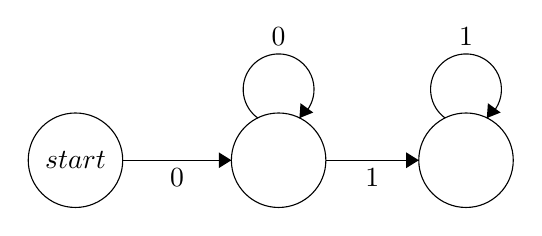
\begin{tikzpicture}[scale=0.2]
            \tikzstyle{every node}+=[inner sep=0pt]
            \draw [black] (9.1,-16.3) circle (3);
            \draw (9.1,-16.3) node {$start$};
            \draw [black] (22,-16.3) circle (3);
            \draw [black] (33.9,-16.3) circle (3);
            \draw [black] (12.1,-16.3) -- (19,-16.3);
            \fill [black] (19,-16.3) -- (18.2,-15.8) -- (18.2,-16.8);
            \draw (15.55,-16.8) node [below] {$0$};
            \draw [black] (20.677,-13.62) arc (234:-54:2.25);
            \draw (22,-9.05) node [above] {$0$};
            \fill [black] (23.32,-13.62) -- (24.2,-13.27) -- (23.39,-12.68);
            \draw [black] (25,-16.3) -- (30.9,-16.3);
            \fill [black] (30.9,-16.3) -- (30.1,-15.8) -- (30.1,-16.8);
            \draw (27.95,-16.8) node [below] {$1$};
            \draw [black] (32.577,-13.62) arc (234:-54:2.25);
            \draw (33.9,-9.05) node [above] {$1$};
            \fill [black] (35.22,-13.62) -- (36.1,-13.27) -- (35.29,-12.68);
            \end{tikzpicture}
            \end{center}
        \2 $\set*{0^n1^n0^n | n \geq 1}$
    \1 给定$\Sigma$, 讨论语言的结构与表示
        \2 $\set*{xx|x \in \Sigma^+} = \set*{a_1a_2\dots a_na_1a_2 \dots a_n|a_1,a_2,\dots,a_n \in \Sigma, n \geq 1}$
        \2 $\set*{xx^T | x \in \Sigma^+}$
        \2 $\set*{xx^Tw | x,w \in \Sigma^+} \\ 
            = \set*{a_1a_2\dots a_n \dots a_1 b_1 \dots b_m | a_1,\dots, a_n, b_1, \dots, b_m \in \Sigma, n,m \geq 1}$
        \2 $\set*{xwx^T|x, w \in \Sigma^+}  \\ 
            = \set*{a_1 \dots a_n b_1 b_2 \dots b_n a_n \dots a_1 | a_1,\dots,a_n,b_1,\dots,b_m \in \Sigma, n,m \geq 1} \\
            = \set*{a a_1 \dots a_n a | a, a_1, a_2, \dots, a_n \in \Sigma, n \geq 1}
            $
\end{outline}

\section{第二章\ 文法} 
\subsection{启示}
\begin{outline}
    \1 对无穷对象的描述
        \2 $\set*{0^n | n \geq 1}$
            \3 $0$ 是 $S$的元素
            \3 $\forall x \in S, x0 \in S$
            \3 $S \to 0$
            \3 $S \to S0$
        \2 $\set*{0^n1^m | n, m \geq 1}$
            \3 $0 \in S$ \\
               $\forall x \in S, 0x, x1 \in S$
            \3 $S \to 01$ \\
               $S \to 0S | S1$
            \3 $S \to S_1S_2$ \\
               $S_1 \to 0$ \\
               $S_1 \to S_10$ \\
               $S_2 \to 0$ \\
               $S_2 \to S_20$
        \2 $\set*{0,1}^*$
            \3 $\epsilon \in S$ \\
               $\forall x \in S, 0x, 1x \in S$
            \3 $S \to \epsilon$ \\
               $S \to 0S $\\
               $S \to 1S $
        \2 $\set*{0,1}^*\set*{11}\set*{0,1}^*$
            \3 $11 \in S$ \\
               $\forall x \in S, 0x, 1x, x0, x1 \in S$
            \3 $S \to 11$ \\
               $S \to 0S | 1S | S0 | S1$
    \1 如何定义中缀表达式:递归
        \2 描述:
            \3 $ident$是表达式
            \3 表达式加表达式是表达式
            \3 表达式减表达式是表达式
            \3 表达式乘表达式是表达式
            \3 表达式除表达式是表达式
            \3 表达式加括号是表达式
        \2 定义:
            \3 表达式\emph{定义为}标识符
            \3 表达式\emph{定义为}表达式$+$表达式
            \3 表达式\emph{定义为}表达式$-$表达式
            \3 表达式\emph{定义为}表达式$\times$表达式
            \3 表达式\emph{定义为}表达式$\div$表达式
            \3 表达式\emph{定义为}(表达式)
        \2 符号化 \par
               $E \to ident$ \\
               $E \to E + E$ \\
               $E \to E - E$ \\
               $E \to E \times E$ \\
               $E \to E \div E$ \\
               $E \to (E)$
        \2 表示优先级
            \3 因子是标识符
            \3 因子是括号的表达式
            \3 项是因子
            \3 项是因子$*/$因子
            \3 表达式是项
            \3 表达式是表达式$+-$表达式
        \2 符号化 
            \3 Variables: $E, T, F$
            \3 Terminals: $+ - \times \div ident ( )$
            \3 Products:  \\
                $E \to T + T$ \\
                $E \to T - T$ \\
                $E \to T$ \\
                $T \to F \times F$ \\
                $T \to F \div F$ \\
                $T \to F $ \\
                $F \to ident$ \\
                $F \to (E)$
            \3 Start Symbol: $E$
\end{outline}
\subsection{形式定义}
\begin{definition}
    文法(Grammar)G是一个四元组
    $$
        G = (V, T, P, S)
    $$
    其中,

    V--- \emph{变量(Variable)}的非空有穷集。$\forall A \in V$,
    $A$叫做语法变量(syntactic variable),也叫非终极符号(nonterminal)。
    
    T--- \emph{终极符(Terminal)}的非空有穷集。$\forall a \in T$,
    $a$叫做终极符。 $V \cup T = \emptyset$。

    P--- \emph{产生式(Production)}的非空有穷集。对于$a \to b$,
    $a$是\emph{左部},$b$是\emph{右部}。

    S--- $S \in V$,文法G的\emph{开始符号(Start symbol)}。
\end{definition}

约定:
\begin{outline}
    \1 只写产生式,第一个产生式的左部为开始符号
    \1 对一组有相同左部的产生式 \\
        $\alpha \to \beta_1, \alpha \to \beta_2, \alpha \to \beta_3, \dots$
        可以记为 $\alpha \to \beta_1 | \beta_2 | \beta_3 \dots$
        $\beta_1 , \beta_2 , \beta_3$称为\emph{候选式}(Candidate)
    \1 形如$\alpha \to \epsilon$的产生式叫做空产生式,也可叫做$\epsilon$产生式
    \1 符号
        \2 英文大写字母为\emph{语法变量}
        \2 英文小写字母为\emph{终结符号}
        \2 英文较后的大写字母为\emph{语法变量或者终极符号}
        \2 英文较后的大写字母为\emph{终极符号行}
        \2 希腊字母表示\emph{语法变量和终极符号组成的行}
\end{outline}

\begin{definition}
    设$G = (V,T,P,S)$是一个文法,如果
    $\alpha \to \beta\in P, \gamma,\delta  \in (V \cup T)$,则称
    $\gamma\alpha\delta$在$G$中\emph{直接推导}(Derivation)出$\gamma\beta\delta$,记作
    $\gamma\alpha\delta \underset{G} \Rightarrow \gamma\beta\delta$。

    于此相对应,$\gamma\beta\delta$归约到$\gamma\alpha\delta$,简称$\beta$归约为$\alpha$。

    $\underset{G} \Rightarrow$ 是$\left( V \cup T \right)^*$上的二元关系。
\end{definition}

\begin{definition}对于文法$G$:

    $\underset{G}{\overset{n}\Longrightarrow } = \left(\underset{G} \Rightarrow \right)^n $ 

    $\underset{G}{\overset{*}\Longrightarrow } = \left(\underset{G} \Rightarrow \right)^* $

    $\underset{G}{\overset{=}\Longrightarrow } = \left(\underset{G} \Rightarrow \right)^+ $

    当只有唯一的文法$G$时,可以省略$G$:$\overset{n}\Longrightarrow, \overset{*}\Longrightarrow, \overset{+}\Longrightarrow$

\end{definition}

\begin{definition}
    对于语言$G = (V, T, P, S)$:

    语法范畴A $L(A) = \set*{w | w \in T^* \text{且} A \overset{*}\Rightarrow w}$

    语言(Language) $L(G) = \set*{w | w \in T^* \text{且} S \overset{*}\Rightarrow w}$

    句子(Sentence) $\forall w \in L(G)$

    句型(Sentential Form) $\forall \alpha \in (V \cup T)^*$, 
    如果$S \overset{*}\Rightarrow \alpha$,则称$\alpha$是$G$产生的一个句型。
    
\end{definition}

\begin{definition}
    对于文法 $G_1, G_2$,如果$L(G_1) = L(G_2)$,则称$G_1$与$G_2$等价。
\end{definition}

\subsection{文法的构造}
\begin{outline}
    \1 $L(G) = \set*{0,1,00,11}$
        \2 $G_1: S \to 0 | 1 | 00 | 11$
        \2 $G_2: S \to A | B | AA | BB, A \to 0, B \to 1$
        \2 $G_3: S \to 0 | 1 | 0A | 1B, A \to 0, B \to 1$
        \2 $G_4: S \to A | B | AA | BB, A \to 0, B \to 1, C \to 1$
    \1 $\set*{x | x \text{是至少3个1的0,1串}}$
        \2 $G: S \to A1A1A1A, A \to \epsilon| 0A| 1A$
        \2 $G: S \to A1A1A1B, A \to \epsilon | 0A, B \to \epsilon | 0B | 1B$
        \2 $G: S \to AAAB, A \to 1 | 0A, B \to \epsilon | 0B | 1B$
\end{outline}

\subsection{文法的乔姆斯体系}
\begin{definition}
    对于文法$G = (V,T,P,S)$: \\
    G叫做0型文法,Type 0 Grammar,也叫短语结构文法(PSG,Phrase Structure Grammar) \\
    $L(G)$是0型语言,也叫短结构语言,可递归枚举集。
\end{definition}
\begin{definition}
    对于0型文法文法$G = (V,T,P,S)$: \\
    如果对于$\forall \alpha \to \beta \in P$,均有$|\beta| \geq |\alpha|$,
    则G是1型文法,或上下文有关文法。
\end{definition}
\begin{definition}
    对于1型文法文法$G = (V,T,P,S)$: \\
    如果对于$\forall \alpha \to \beta \in P$,均有$|\beta| \geq |\alpha|$,
    并且$\alpha \in V$
    则G是2型文法,或上下文无关文法。
\end{definition}
\begin{definition}
    对于2型文法文法$G = (V,T,P,S)$: \\
    如果对于$\forall \alpha \to \beta \in P$: \\
    如果形如$A \to wB$和$A \to w$,其中$A,B \in V, w \in T^+$:G是右线性文法。 \\
    如果形如$A \to Bw$和$A \to w$,其中$A,B \in V, w \in T^+$:G是左线性文法。 \\
    则G是3型文法,或正则文法。
\end{definition}

\subsection{空产生式}
允许在CSG,CFG,RG文法中存在空产生式。 

允许在CSL,CFL,RL语言中存在空语句。

特点:
\begin{outline}
    \1 对于$\forall$右线性文法$G_1$,$\exists$ 左线性文法 $G_2$ 使得 
    $L(G_1) = L(G_2)$
    \1 对于$\forall$左线性文法$G_1$,$\exists$ 右线性文法 $G_2$ 使得 
    $L(G_1) = L(G_2)$ \\
        所以,某种意义上二者等价。其中,\emph{左线性文法的表述好。}\\
        \hl{\emph{左递归}?}
        \emph{线性文法不是正则文法!}
    \1 $\forall G, \exists G', L(G') = L(G)$,但是$G'$中的开好似符号不出现在任何
    产生式的右部,且在$\epsilon \in L(G')$时,$G'$中只有$S' \to \epsilon$这样一个
    $\epsilon$产生式。
\end{outline}

\subsubsection{语言运算}
给定上下文无关文法$G_1,G_2$,构造$G$使得:
\begin{outline}[enumerate]
    \1 $L(G) = L(G_1)L(G_2)$ \\
        其中$V_1 \cup V_2 = \emptyset$, $S \notin V_1 \cup V_2$

        $G = (V_1 \cup V_2 \cup {S}, T, P_1 \cup P_2 \cup {S \to S_1S_2}, S)$

    \1 $L(G) = L(G_1) \cup L(G_2)$

        $G_\cup = (V_1 \cup V_2 \cup {S}, T, P_1 \cup P_2 \cup P_3, S)$ \\
        $P_3 = \set*{S \to S_1 | S_2}$

    \1 $L(G) = L(G_1)^*$

        $G_* = \paren*{V_1 \cup \set*{S}, T, P_1 \cup P_2, S}$ \\
        $P_2 = \set*{S \to \epsilon | SS_1}$

\end{outline}

给定RG $G_1,G_2$,构造RG $G$使得:
\begin{outline}[enumerate]
    \1 $L(G) = L(G_1)L(G_2)$ \\
        其中$V_1 \cup V_2 = \emptyset$, $S \notin V_1 \cup V_2$

        $\begin{aligned}
            S_1  & \tto a_1A_1 \\
                 & \tto a_1a_2\dots a_{n-1}A_n  \\
                 & \tto a_1a_2\dots a_nS_2
        \end{aligned}$
        所以,我们需要改造$P_1$。

        $G = (V_1 \cup V_2 \cup {S}, T, P_1' \cup P_2 \cup P_3, S_1)$

        $P_1' = \set*{A \to a B | A \to a B \in P_1}$
        
        $P_3 = \set*{A \to a S_2 | A \to a \in P_1}$

    \1 $L(G) = L(G_1) \cup L(G_2)$

        $G_\cup = (V_1 \cup V_2 \cup {S}, T, P_1 \cup P_2 \cup P, S)$ \\
        $\begin{aligned}
            P & = \set*{S \to \alpha | S_1 \to \alpha \in P_1} \\
            & \cup \set*{S \to \alpha | S_2 \to \alpha \in P_2} \\
        \end{aligned}$

    \1 $L(G) = L(G_1)^*$

        \hl{自己想!}
\end{outline}

例子:

\begin{outline}[enumerate]
    \1 设$L = \set*{x | 101 \text{ in } x}$,构造 $G, L(G) = L$。

    朴素构造:$\begin{cases}
        S \to A 101 A \\
        A \to \epsilon | 0A | 1A
    \end{cases}$
    
    正则构造:$\begin{cases}
        S \to 0S | 1A \\
        A \to 0B | 1A \\
        B \to 1C | 0S \\
        C \to 0C | 1C | \epsilon
    \end{cases}$

    \1 构造$G$使$L(G) = \set*{x | 101 \text{ not in } x}$

    正则构造:$\begin{cases}
        S \to 0S | 1A \\
        A \to 0B | 1A \\
        B \to 0S | \epsilon\\
    \end{cases}$
\end{outline}



\subsection{小结}


习题: p67 3,4,8.2,8.6,10.3,11.3

\section{有穷状态自动机 Finite Automata}

习题:p103 2.4, 2.11; p104 7, 10.6

\subsection{FA的基本定义}
\begin{figure}[H]
    \centering
    \caption{有穷状态自动机}
    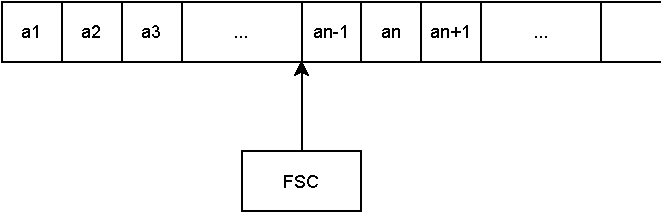
\includegraphics{FA}
\end{figure}

\begin{definition}
    $M = (Q, \Sigma, \delta, q_0, F)$,其中:

    \begin{description}
        \item[$Q$]:状态的有穷集合
        \item[$\Sigma$]: 输入字母表
        \item[$\delta$]: 状态转义函数\\
            $Q\times\Sigma \to Q$。 $\forall (q,a) \in Q\times\Sigma$,
            $\delta(q,a) = p$表示$M$在状态$q$读入一个字符$a$,状态改为$p$并
            指向下一个字符。
        \item[$q_0$]:开始状态
        \item[$F$]: 终止状态 
    \end{description}
\end{definition}
\begin{definition}
    有穷状态自动机$M = (Q, \Sigma, \delta, q_0, F)$:

    状态转移图是满足如下条件的有向图。
    \begin{enumerate}
        \item 对于$q \in Q$, $q$是一个顶点
        \item $\forall (q,a) \in \delta$, $q$到$p$有一条标记为$a$的弧。
        \item 标有S的箭头所指的状态为开始状态。
        \item 用双圈标记结束状态。
    \end{enumerate}

    扩展$\delta$为$\hat{\delta}: Q \times \Sigma^* \to Q$
    \begin{enumerate}
        \item $\hat{\delta}(q,\epsilon) = q$
        \item $\hat{\delta}(q, wa) = \delta(\hat{\delta}(q,w), a)$
    \end{enumerate}
    注意到 $Q \time \Sigma \subset Q \times \Sigma^*$,
    且对$\forall (q, a) \in Q \times \Sigma$,$\hat{\delta}(q, a) = \delta(q, a)$
    所以,不用区分$\delta$与$\hat{\delta}$。 \\
    $\delta$是$Q \times \Sigma^* \to Q$上的映射。
\end{definition}

\begin{definition}
    有穷状态自动机$M = (Q, \Sigma, \delta, q_0, F)$识别的语言:
    $L(M) = \set*{x | \delta(q_0, x) \in F}$
\end{definition}

\begin{definition}
    对于有穷状态自动机$M_1, M_2$:若有$L(M_1) = L(M_2)$,则称二者等价。
\end{definition}

\begin{definition}
    对于有穷自动状态机$M = (Q, \Sigma, \delta, q_0, F)$,$set(q) = 
    \set*{x | \delta(q_0, x) = q}$

    所以有:$\Sigma^* = \bigcup_{q \in Q}set(q)$;
    $\forall q,p \in Q, q \ne p, set(q) \cap set(p) = \emptyset $

    同时,如果$Q$中不存在不可达状态,则$set(q_0), set(q_1) \dots$
    是$\Sigma^*$的一个划分。
\end{definition}

\begin{definition}
    \begin{align*}
        x R_M y & \iff \delta(q_0, x) = \delta(q_0, y) \\
            & \iff \exists q \in Q, x, y \in set(q)
    \end{align*}
\end{definition}

\begin{example}
    构造$M$,使得$L(M) = \set*{x000 | x \in \set*{0,1}^*}$。 
    \begin{center}
        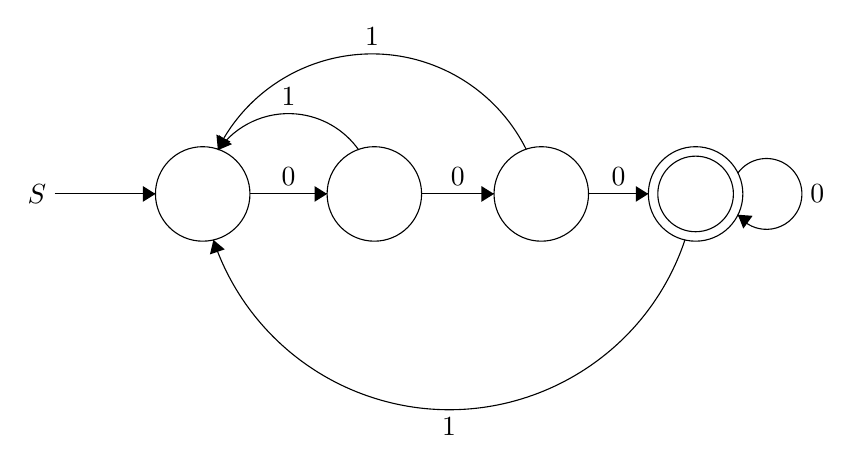
\begin{tikzpicture}[scale=0.2]
            \tikzstyle{every node}+=[inner sep=0pt]
            \draw [black] (13.8,-12.7) circle (3);
            \draw [black] (24.7,-12.7) circle (3);
            \draw [black] (35.3,-12.7) circle (3);
            \draw [black] (45.1,-12.7) circle (3);
            \draw [black] (45.1,-12.7) circle (2.4);
            \draw [black] (16.8,-12.7) -- (21.7,-12.7);
            \fill [black] (21.7,-12.7) -- (20.9,-12.2) -- (20.9,-13.2);
            \draw (19.25,-12.2) node [above] {$0$};
            \draw [black] (27.7,-12.7) -- (32.3,-12.7);
            \fill [black] (32.3,-12.7) -- (31.5,-12.2) -- (31.5,-13.2);
            \draw (30,-12.2) node [above] {$0$};
            \draw [black] (38.3,-12.7) -- (42.1,-12.7);
            \fill [black] (42.1,-12.7) -- (41.3,-12.2) -- (41.3,-13.2);
            \draw (40.2,-12.2) node [above] {$0$};
            \draw [black] (14.789,-9.908) arc (144.75241:35.24759:5.462);
            \fill [black] (14.79,-9.91) -- (15.66,-9.54) -- (14.84,-8.97);
            \draw (19.25,-7.1) node [above] {$1$};
            \draw [black] (14.757,-9.867) arc (153.48523:26.51477:10.944);
            \fill [black] (14.76,-9.87) -- (15.56,-9.37) -- (14.67,-8.93);
            \draw (24.55,-3.31) node [above] {$1$};
            \draw [black] (44.424,-15.618) arc (-18.48859:-161.51141:15.789);
            \fill [black] (14.48,-15.62) -- (14.26,-16.54) -- (15.2,-16.22);
            \draw (29.45,-26.9) node [below] {$1$};
            \draw [black] (4.4,-12.7) -- (10.8,-12.7);
            \draw (3.9,-12.7) node [left] {$S$};
            \fill [black] (10.8,-12.7) -- (10,-12.2) -- (10,-13.2);
            \draw [black] (47.78,-11.377) arc (144:-144:2.25);
            \draw (52.35,-12.7) node [right] {$0$};
            \fill [black] (47.78,-14.02) -- (48.13,-14.9) -- (48.72,-14.09);
            \end{tikzpicture}
    \end{center}
\end{example}
\begin{example}
    
    构造$M$,使得$L(M) = \set*{0x0 | x \in \set*{0,1}^*}$。 


    \begin{center}
        \begin{tikzpicture}[scale=0.2]
        \tikzstyle{every node}+=[inner sep=0pt]
        \draw [black] (24,-10.8) circle (3);
        \draw (24,-10.8) node {偶0};
        \draw [black] (50.8,-10.8) circle (3);
        \draw (50.8,-10.8) node {奇0};
        \draw [black] (50.8,-10.8) circle (2.4);
        \draw [black] (50.8,-31.5) circle (3);
        \draw (50.8,-31.5) node {偶1};
        \draw [black] (50.8,-31.5) circle (2.4);
        \draw [black] (24,-31.5) circle (3);
        \draw (24,-31.5) node {奇1};
        \draw [black] (37.4,-21.3) circle (3);
        \draw (37.4,-21.3) node {$\epsilon$};
        \draw [black] (31,-16.7) -- (34.96,-19.55);
        \draw (30.41,-15.32) node [left] {$S$};
        \fill [black] (34.96,-19.55) -- (34.61,-18.68) -- (34.02,-19.49);
        \draw [black] (26.895,-10.014) arc (103.30426:76.69574:45.651);
        \fill [black] (47.91,-10.01) -- (47.24,-9.34) -- (47.01,-10.32);
        \draw (37.4,-8.29) node [above] {$0$};
        \draw [black] (25.056,-13.606) arc (17.24582:-17.24582:25.446);
        \fill [black] (25.06,-28.69) -- (25.77,-28.08) -- (24.82,-27.78);
        \draw (26.7,-21.15) node [right] {$1$};
        \draw [black] (47.926,-11.657) arc (-75.44172:-104.55828:41.875);
        \fill [black] (26.87,-11.66) -- (27.52,-12.34) -- (27.77,-11.37);
        \draw (37.4,-13.5) node [below] {$0$};
        \draw [black] (51.962,-13.563) arc (19.10726:-19.10726:23.177);
        \fill [black] (51.96,-28.74) -- (52.7,-28.14) -- (51.75,-27.82);
        \draw (53.74,-21.15) node [right] {$1$};
        \draw [black] (49.689,-28.715) arc (-161.799:-198.201:24.221);
        \fill [black] (49.69,-13.58) -- (48.96,-14.19) -- (49.91,-14.5);
        \draw (47.98,-21.15) node [left] {$0$};
        \draw [black] (47.859,-32.092) arc (-80.03528:-99.96472:60.444);
        \fill [black] (26.94,-32.09) -- (27.64,-32.72) -- (27.82,-31.74);
        \draw (37.4,-33.5) node [below] {$1$};
        \draw [black] (26.906,-30.755) arc (102.59162:77.40838:48.139);
        \fill [black] (47.89,-30.76) -- (47.22,-30.09) -- (47,-31.07);
        \draw (37.4,-29.1) node [above] {$1$};
        \draw [black] (22.854,-28.73) arc (-161.18818:-198.81182:23.505);
        \fill [black] (22.85,-13.57) -- (22.12,-14.17) -- (23.07,-14.49);
        \draw (21.1,-21.15) node [left] {$0$};
        \draw [black] (35.01,-23.12) -- (26.39,-29.68);
        \fill [black] (26.39,-29.68) -- (27.33,-29.6) -- (26.72,-28.8);
        \draw (29.73,-25.9) node [above] {$1$};
        \draw [black] (39.76,-19.45) -- (48.44,-12.65);
        \fill [black] (48.44,-12.65) -- (47.5,-12.75) -- (48.12,-13.54);
        \draw (45.07,-16.55) node [below] {$0$};
        \end{tikzpicture}
    \end{center}
        
\end{example}

\begin{example}
    构造$M$,使得$L(M) = \set*{x | \text{x看作二进制时,}x \mod 3 = 1}$。 
\begin{center}
    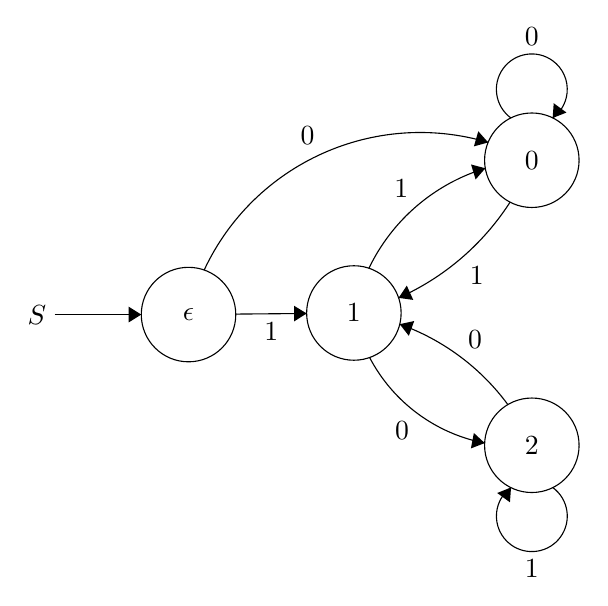
\begin{tikzpicture}[scale=0.2]
    \tikzstyle{every node}+=[inner sep=0pt]
    \draw [black] (38.9,-19.1) circle (3);
    \draw (38.9,-19.1) node {$0$};
    \draw [black] (27.6,-28.8) circle (3);
    \draw (27.6,-28.8) node {$1$};
    \draw [black] (38.9,-37.2) circle (3);
    \draw (38.9,-37.2) node {$2$};
    \draw [black] (17.1,-28.9) circle (3);
    \draw (17.1,-28.9) node {$\epsilon$};
    \draw [black] (28.553,-25.963) arc (154.34808:106.93797:12.128);
    \fill [black] (35.95,-19.61) -- (35.04,-19.37) -- (35.33,-20.32);
    \draw (30.61,-21.52) node [above] {$1$};
    \draw [black] (35.913,-37.06) arc (-100.87688:-152.3746:10.496);
    \fill [black] (35.91,-37.06) -- (35.22,-36.42) -- (35.03,-37.4);
    \draw (30.66,-35.67) node [below] {$0$};
    \draw [black] (37.52,-21.759) arc (-32.71252:-66.00143:16.293);
    \fill [black] (30.44,-27.84) -- (31.37,-27.97) -- (30.96,-27.06);
    \draw (35.4,-25.81) node [below] {$1$};
    \draw [black] (37.577,-16.42) arc (234:-54:2.25);
    \draw (38.9,-11.85) node [above] {$0$};
    \fill [black] (40.22,-16.42) -- (41.1,-16.07) -- (40.29,-15.48);
    \draw [black] (40.223,-39.88) arc (54:-234:2.25);
    \draw (38.9,-44.45) node [below] {$1$};
    \fill [black] (37.58,-39.88) -- (36.7,-40.23) -- (37.51,-40.82);
    \draw [black] (30.509,-29.512) arc (70.37322:36.37529:14.642);
    \fill [black] (30.51,-29.51) -- (31.09,-30.25) -- (31.43,-29.31);
    \draw (35.3,-31.06) node [above] {$0$};
    \draw [black] (8.6,-28.9) -- (14.1,-28.9);
    \draw (8.1,-28.9) node [left] {$S$};
    \fill [black] (14.1,-28.9) -- (13.3,-28.4) -- (13.3,-29.4);
    \draw [black] (20.1,-28.87) -- (24.6,-28.83);
    \fill [black] (24.6,-28.83) -- (23.8,-28.34) -- (23.8,-29.34);
    \draw (22.35,-29.36) node [below] {$1$};
    \draw [black] (18.093,-26.074) arc (154.9625:73.44927:15.144);
    \fill [black] (36.13,-17.97) -- (35.5,-17.26) -- (35.22,-18.22);
    \draw (24.66,-18.16) node [above] {$0$};
    \end{tikzpicture}
\end{center}
\end{example}

\begin{example}
    对于FSA $M = (Q, \Sigma, \delta, q_0, F)$,构造FA 
    $M'$使得$L(M') = \Sigma^* - L(M)$

    $M' = (Q, \Sigma, \delta, q_0, \complement_QF )$
\end{example}

\begin{example}
    给定 $\begin{cases}
        M_1 = (Q_1, \Sigma, \delta_1, q_{01}, F_1) \\
        M_2 = (Q_2, \Sigma, \delta_2, q_{02}, F_2)
    \end{cases}$
    构造:
    \begin{outline}
        \1 $M_3$使得$L(M_3) = L(M_1) \cap L(M_2)$
        \1 $M_3$使得$L(M_3) = L(M_1) \cup L(M_2)$
    \end{outline}
\end{example}

\begin{example}
    构造$M$,使得$L(M) = \set*{x | x \in \set*{0,1}^+ \mathrm{and} \text{ x的第三个字符是1}}$。 

    \begin{center}
        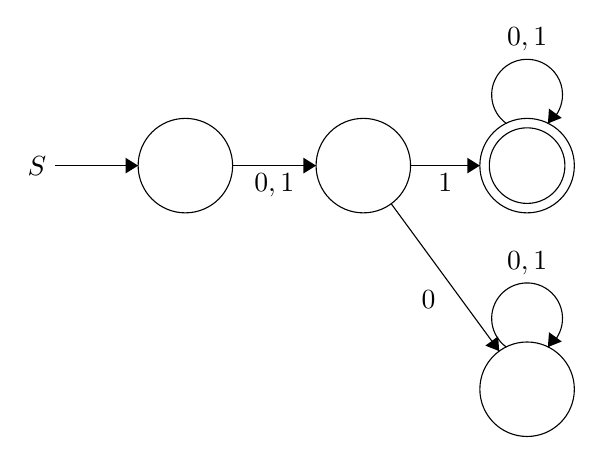
\begin{tikzpicture}[scale=0.2]
        \tikzstyle{every node}+=[inner sep=0pt]
        \draw [black] (14.1,-24.5) circle (3);
        \draw [black] (25.4,-24.5) circle (3);
        \draw [black] (35.8,-24.5) circle (3);
        \draw [black] (35.8,-24.5) circle (2.4);
        \draw [black] (35.8,-38.7) circle (3);
        \draw [black] (17.1,-24.5) -- (22.4,-24.5);
        \fill [black] (22.4,-24.5) -- (21.6,-24) -- (21.6,-25);
        \draw (19.75,-25) node [below] {$0,1$};
        \draw [black] (28.4,-24.5) -- (32.8,-24.5);
        \fill [black] (32.8,-24.5) -- (32,-24) -- (32,-25);
        \draw (30.6,-25) node [below] {$1$};
        \draw [black] (27.17,-26.92) -- (34.03,-36.28);
        \fill [black] (34.03,-36.28) -- (33.96,-35.34) -- (33.15,-35.93);
        \draw (30.02,-32.99) node [left] {$0$};
        \draw [black] (34.477,-21.82) arc (234:-54:2.25);
        \draw (35.8,-17.25) node [above] {$0,1$};
        \fill [black] (37.12,-21.82) -- (38,-21.47) -- (37.19,-20.88);
        \draw [black] (5.8,-24.5) -- (11.1,-24.5);
        \draw (5.3,-24.5) node [left] {$S$};
        \fill [black] (11.1,-24.5) -- (10.3,-24) -- (10.3,-25);
        \draw [black] (34.477,-36.02) arc (234:-54:2.25);
        \draw (35.8,-31.45) node [above] {$0,1$};
        \fill [black] (37.12,-36.02) -- (38,-35.67) -- (37.19,-35.08);
        \end{tikzpicture}
    \end{center}        
\end{example}
\begin{example}
    构造$M$,使得$L(M) = \set*{x | x \in \set*{0,1}^+ \mathrm{and} \text{ x的倒数第三个字符是1}}$。 
    \begin{center}
        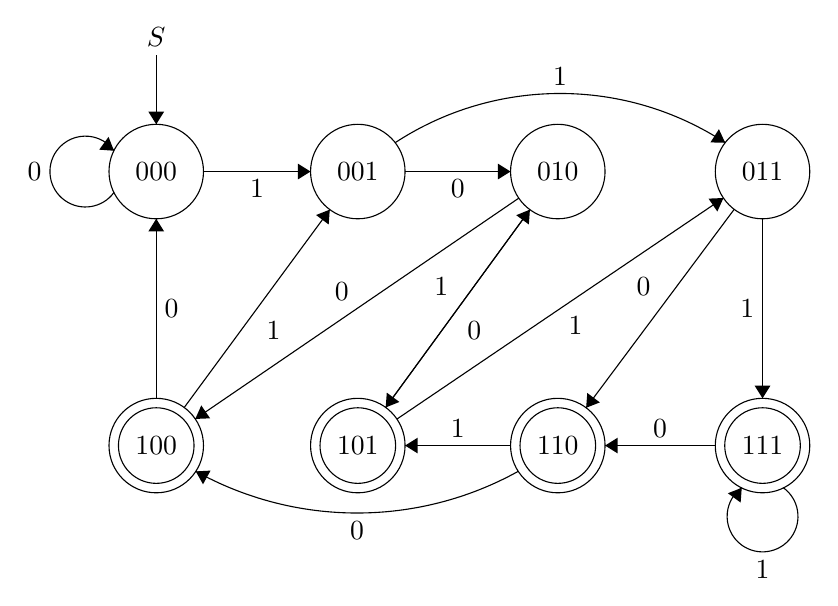
\begin{tikzpicture}[scale=0.2]
        \tikzstyle{every node}+=[inner sep=0pt]
        \draw [black] (30.6,-16.2) circle (3);
        \draw (30.6,-16.2) node {$000$};
        \draw [black] (43.4,-16.2) circle (3);
        \draw (43.4,-16.2) node {$001$};
        \draw [black] (56.1,-16.2) circle (3);
        \draw (56.1,-16.2) node {$010$};
        \draw [black] (69.1,-16.2) circle (3);
        \draw (69.1,-16.2) node {$011$};
        \draw [black] (30.6,-33.6) circle (3);
        \draw (30.6,-33.6) node {$100$};
        \draw [black] (30.6,-33.6) circle (2.4);
        \draw [black] (43.4,-33.6) circle (3);
        \draw (43.4,-33.6) node {$101$};
        \draw [black] (43.4,-33.6) circle (2.4);
        \draw [black] (56.1,-33.6) circle (3);
        \draw (56.1,-33.6) node {$110$};
        \draw [black] (56.1,-33.6) circle (2.4);
        \draw [black] (69.1,-33.6) circle (3);
        \draw (69.1,-33.6) node {$111$};
        \draw [black] (69.1,-33.6) circle (2.4);
        \draw [black] (33.6,-16.2) -- (40.4,-16.2);
        \fill [black] (40.4,-16.2) -- (39.6,-15.7) -- (39.6,-16.7);
        \draw (37,-16.7) node [below] {$1$};
        \draw [black] (27.92,-17.523) arc (-36:-324:2.25);
        \draw (23.35,-16.2) node [left] {$0$};
        \fill [black] (27.92,-14.88) -- (27.57,-14) -- (26.98,-14.81);
        \draw [black] (45.771,-14.367) arc (123.20907:56.79093:19.133);
        \fill [black] (66.73,-14.37) -- (66.33,-13.51) -- (65.79,-14.35);
        \draw (56.25,-10.74) node [above] {$1$};
        \draw [black] (46.4,-16.2) -- (53.1,-16.2);
        \fill [black] (53.1,-16.2) -- (52.3,-15.7) -- (52.3,-16.7);
        \draw (49.75,-16.7) node [below] {$0$};
        \draw [black] (54.33,-18.62) -- (45.17,-31.18);
        \fill [black] (45.17,-31.18) -- (46.04,-30.83) -- (45.24,-30.24);
        \draw (49.17,-23.52) node [left] {$1$};
        \draw [black] (53.62,-17.89) -- (33.08,-31.91);
        \fill [black] (33.08,-31.91) -- (34.02,-31.87) -- (33.46,-31.05);
        \draw (42.38,-24.4) node [above] {$0$};
        \draw [black] (69.1,-19.2) -- (69.1,-30.6);
        \fill [black] (69.1,-30.6) -- (69.6,-29.8) -- (68.6,-29.8);
        \draw (68.6,-24.9) node [left] {$1$};
        \draw [black] (67.3,-18.6) -- (57.9,-31.2);
        \fill [black] (57.9,-31.2) -- (58.77,-30.86) -- (57.97,-30.26);
        \draw (62.02,-23.5) node [left] {$0$};
        \draw [black] (30.6,-30.6) -- (30.6,-19.2);
        \fill [black] (30.6,-19.2) -- (30.1,-20) -- (31.1,-20);
        \draw (31.1,-24.9) node [right] {$0$};
        \draw [black] (32.38,-31.18) -- (41.62,-18.62);
        \fill [black] (41.62,-18.62) -- (40.75,-18.96) -- (41.55,-19.56);
        \draw (37.58,-26.29) node [right] {$1$};
        \draw [black] (45.88,-31.92) -- (66.62,-17.88);
        \fill [black] (66.62,-17.88) -- (65.67,-17.92) -- (66.23,-18.74);
        \draw (57.22,-25.4) node [below] {$1$};
        \draw [black] (45.17,-31.18) -- (54.33,-18.62);
        \fill [black] (54.33,-18.62) -- (53.46,-18.97) -- (54.26,-19.56);
        \draw (50.33,-26.28) node [right] {$0$};
        \draw [black] (53.1,-33.6) -- (46.4,-33.6);
        \fill [black] (46.4,-33.6) -- (47.2,-34.1) -- (47.2,-33.1);
        \draw (49.75,-33.1) node [above] {$1$};
        \draw [black] (53.588,-35.236) arc (-60.99857:-119.00143:21.117);
        \fill [black] (33.11,-35.24) -- (33.57,-36.06) -- (34.05,-35.19);
        \draw (43.35,-38.38) node [below] {$0$};
        \draw [black] (70.423,-36.28) arc (54:-234:2.25);
        \draw (69.1,-40.85) node [below] {$1$};
        \fill [black] (67.78,-36.28) -- (66.9,-36.63) -- (67.71,-37.22);
        \draw [black] (66.1,-33.6) -- (59.1,-33.6);
        \fill [black] (59.1,-33.6) -- (59.9,-34.1) -- (59.9,-33.1);
        \draw (62.6,-33.1) node [above] {$0$};
        \draw [black] (30.6,-8.8) -- (30.6,-13.2);
        \draw (30.6,-8.3) node [above] {$S$};
        \fill [black] (30.6,-13.2) -- (31.1,-12.4) -- (30.1,-12.4);
        \end{tikzpicture}
        \end{center} 
\end{example}
\subsection{NFA 不确定的有穷状态自动机}
\begin{definition}
    NFA $M = (Q, \Sigma, \delta, q_0, F)$,其中:

    $Q, \Sigma, q_0, F$ 同 FA。

    $\delta$: $Q \times \Sigma \to 2^Q$ (幂集),\\
    $\delta(q, a) = \set*{p_1, p_2, \dots, p_n}$表示M
    在状态$q$读入$a$可以选择进入$p_i$

    扩展$\delta$为$\hat{\delta}: Q \times \Sigma^* \to 2^Q$
   
    \begin{align*}
            \hat{\delta}(q,\epsilon)  & = \set*{q} \\
            \hat{\delta}(q, wa) & = \bigcup_{q_0 \in \hat{\delta}(q,w)}\delta(q_0, a)
    \end{align*}

    进一步拓展: $\hat{\delta}: 2^Q \times \Sigma^* \to 2^Q$

    \begin{align*}
        \hat{\delta}(P, x) = \bigcup_{p \in P}\hat{\delta}(p, x)
    \end{align*}

    注意到 $Q \times \Sigma \subset 2^Q \times \Sigma^*$,
    且对$\forall (q, a) \in Q \times \Sigma^*$,$\hat{\delta}(q, a) = \delta(q, a)$
    所以不用区分$\delta$与$\hat{\delta}$。 

    $\delta$是$Q \times \Sigma^* \to Q$上的映射。
\end{definition}

\begin{example}
    构造NFA $M$, 使得$L(M) = \set*{x | \text{x是含110的01串}}$


    \begin{center}
        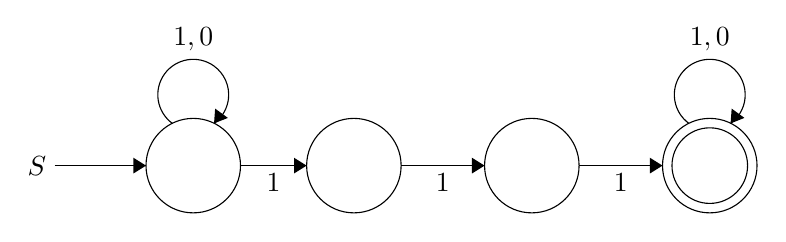
\begin{tikzpicture}[scale=0.2]
        \tikzstyle{every node}+=[inner sep=0pt]
        \draw [black] (15.3,-32.1) circle (3);
        \draw [black] (25.5,-32.1) circle (3);
        \draw [black] (36.8,-32.1) circle (3);
        \draw [black] (48.1,-32.1) circle (3);
        \draw [black] (48.1,-32.1) circle (2.4);
        \draw [black] (18.3,-32.1) -- (22.5,-32.1);
        \fill [black] (22.5,-32.1) -- (21.7,-31.6) -- (21.7,-32.6);
        \draw (20.4,-32.6) node [below] {$1$};
        \draw [black] (28.5,-32.1) -- (33.8,-32.1);
        \fill [black] (33.8,-32.1) -- (33,-31.6) -- (33,-32.6);
        \draw (31.15,-32.6) node [below] {$1$};
        \draw [black] (13.977,-29.42) arc (234:-54:2.25);
        \draw (15.3,-24.85) node [above] {$1,0$};
        \fill [black] (16.62,-29.42) -- (17.5,-29.07) -- (16.69,-28.48);
        \draw [black] (6.5,-32.1) -- (12.3,-32.1);
        \draw (6,-32.1) node [left] {$S$};
        \fill [black] (12.3,-32.1) -- (11.5,-31.6) -- (11.5,-32.6);
        \draw [black] (39.8,-32.1) -- (45.1,-32.1);
        \fill [black] (45.1,-32.1) -- (44.3,-31.6) -- (44.3,-32.6);
        \draw (42.45,-32.6) node [below] {$1$};
        \draw [black] (46.777,-29.42) arc (234:-54:2.25);
        \draw (48.1,-24.85) node [above] {$1,0$};
        \fill [black] (49.42,-29.42) -- (50.3,-29.07) -- (49.49,-28.48);
        \end{tikzpicture}
        \end{center}
\end{example}

\begin{example}
    构造NFA $M$, 使得$L(M) = \set*{x | \text{x是00结尾的01串}}$
    \begin{center}
        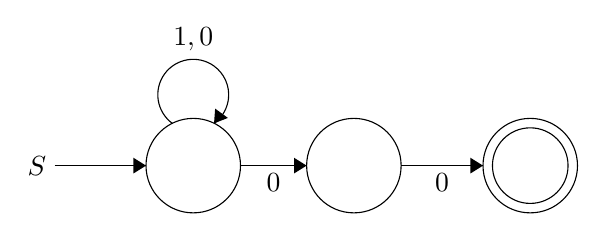
\begin{tikzpicture}[scale=0.2]
        \tikzstyle{every node}+=[inner sep=0pt]
        \draw [black] (15.3,-32.1) circle (3);
        \draw [black] (25.5,-32.1) circle (3);
        \draw [black] (36.7,-32.1) circle (3);
        \draw [black] (36.7,-32.1) circle (2.4);
        \draw [black] (18.3,-32.1) -- (22.5,-32.1);
        \fill [black] (22.5,-32.1) -- (21.7,-31.6) -- (21.7,-32.6);
        \draw (20.4,-32.6) node [below] {$0$};
        \draw [black] (28.5,-32.1) -- (33.7,-32.1);
        \fill [black] (33.7,-32.1) -- (32.9,-31.6) -- (32.9,-32.6);
        \draw (31.1,-32.6) node [below] {$0$};
        \draw [black] (13.977,-29.42) arc (234:-54:2.25);
        \draw (15.3,-24.85) node [above] {$1,0$};
        \fill [black] (16.62,-29.42) -- (17.5,-29.07) -- (16.69,-28.48);
        \draw [black] (6.5,-32.1) -- (12.3,-32.1);
        \draw (6,-32.1) node [left] {$S$};
        \fill [black] (12.3,-32.1) -- (11.5,-31.6) -- (11.5,-32.6);
        \end{tikzpicture}
    \end{center}
\end{example}

\begin{example}
    构造NFA $M$, 使得$L(M) = \set*{x | \text{x是00开头或结尾的01串}}$

    \begin{center}
        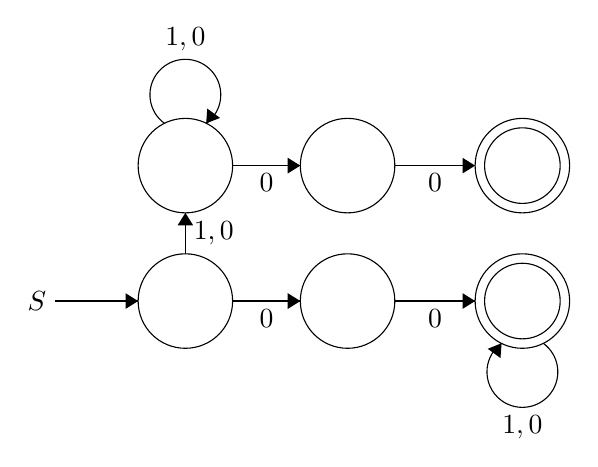
\begin{tikzpicture}[scale=0.2]
        \tikzstyle{every node}+=[inner sep=0pt]
        \draw [black] (15.3,-32.1) circle (3);
        \draw [black] (25.6,-32.1) circle (3);
        \draw [black] (36.7,-32.1) circle (3);
        \draw [black] (36.7,-32.1) circle (2.4);
        \draw [black] (15.3,-40.7) circle (3);
        \draw [black] (25.6,-40.7) circle (3);
        \draw [black] (36.7,-40.7) circle (3);
        \draw [black] (36.7,-40.7) circle (2.4);
        \draw [black] (18.3,-32.1) -- (22.6,-32.1);
        \fill [black] (22.6,-32.1) -- (21.8,-31.6) -- (21.8,-32.6);
        \draw (20.45,-32.6) node [below] {$0$};
        \draw [black] (28.6,-32.1) -- (33.7,-32.1);
        \fill [black] (33.7,-32.1) -- (32.9,-31.6) -- (32.9,-32.6);
        \draw (31.15,-32.6) node [below] {$0$};
        \draw [black] (13.977,-29.42) arc (234:-54:2.25);
        \draw (15.3,-24.85) node [above] {$1,0$};
        \fill [black] (16.62,-29.42) -- (17.5,-29.07) -- (16.69,-28.48);
        \draw [black] (18.3,-40.7) -- (22.6,-40.7);
        \fill [black] (22.6,-40.7) -- (21.8,-40.2) -- (21.8,-41.2);
        \draw (20.45,-41.2) node [below] {$0$};
        \draw [black] (28.6,-40.7) -- (33.7,-40.7);
        \fill [black] (33.7,-40.7) -- (32.9,-40.2) -- (32.9,-41.2);
        \draw (31.15,-41.2) node [below] {$0$};
        \draw [black] (38.023,-43.38) arc (54:-234:2.25);
        \draw (36.7,-47.95) node [below] {$1,0$};
        \fill [black] (35.38,-43.38) -- (34.5,-43.73) -- (35.31,-44.32);
        \draw [black] (15.3,-37.7) -- (15.3,-35.1);
        \fill [black] (15.3,-35.1) -- (14.8,-35.9) -- (15.8,-35.9);
        \draw (15.8,-36.4) node [right] {$1,0$};
        \draw [black] (7,-40.7) -- (12.3,-40.7);
        \draw (6.5,-40.7) node [left] {$S$};
        \fill [black] (12.3,-40.7) -- (11.5,-40.2) -- (11.5,-41.2);
        \end{tikzpicture}
        \end{center}
\end{example}

\begin{theorem}
    NFA与DFA等价。

    证:对于NFA $ M= (Q, \Sigma, \delta, q_0, F)$,构造
    DFA $M' = (2^Q, \Sigma, \delta', [q_0], F')$

    $F'= \set*{[q_1, q_2, \dots, q_n] |
     \set*{q_1, q_2, \dots, q_n} \cap F \ne \emptyset}$

    $\delta'([q_1, q_2, \dots, q_n], a) = 
    [\beta_1, \beta_2, \dots, \beta_n] \iff 
    \delta(\set*{q_1, q_2, \dots, q_n}, a) = \set*{\beta_1, \beta_2, \dots, \beta_n}
    $

    所以,对于$\forall M$ 是NFA,可以构造DFA $M'$
\end{theorem}

\begin{example}
    构造DFA $M$, $L(M) = \set*{0^n1^m2^k | n,m,k \ge 1}$

\begin{center}
    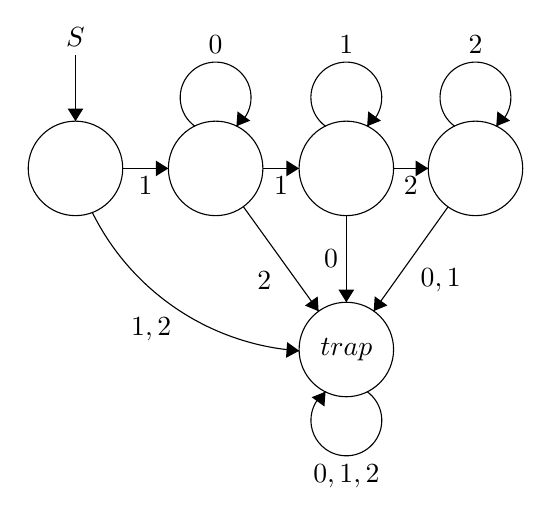
\begin{tikzpicture}[scale=0.2]
    \tikzstyle{every node}+=[inner sep=0pt]
    \draw [black] (19.3,-22.5) circle (3);
    \draw [black] (27.6,-22.5) circle (3);
    \draw [black] (35.8,-22.5) circle (3);
    \draw [black] (27.6,-34) circle (3);
    \draw (27.6,-34) node {$trap$};
    \draw [black] (10.4,-22.5) circle (3);
    \draw [black] (26.277,-19.82) arc (234:-54:2.25);
    \draw (27.6,-15.25) node [above] {$1$};
    \fill [black] (28.92,-19.82) -- (29.8,-19.47) -- (28.99,-18.88);
    \draw [black] (30.6,-22.5) -- (32.8,-22.5);
    \fill [black] (32.8,-22.5) -- (32,-22) -- (32,-23);
    \draw (31.7,-23) node [below] {$2$};
    \draw [black] (22.3,-22.5) -- (24.6,-22.5);
    \fill [black] (24.6,-22.5) -- (23.8,-22) -- (23.8,-23);
    \draw (23.45,-23) node [below] {$1$};
    \draw [black] (17.977,-19.82) arc (234:-54:2.25);
    \draw (19.3,-15.25) node [above] {$0$};
    \fill [black] (20.62,-19.82) -- (21.5,-19.47) -- (20.69,-18.88);
    \draw [black] (34.477,-19.82) arc (234:-54:2.25);
    \draw (35.8,-15.25) node [above] {$2$};
    \fill [black] (37.12,-19.82) -- (38,-19.47) -- (37.19,-18.88);
    \draw [black] (21.06,-24.93) -- (25.84,-31.57);
    \fill [black] (25.84,-31.57) -- (25.78,-30.63) -- (24.97,-31.21);
    \draw (22.86,-29.63) node [left] {$2$};
    \draw [black] (27.6,-25.5) -- (27.6,-31);
    \fill [black] (27.6,-31) -- (28.1,-30.2) -- (27.1,-30.2);
    \draw (27.1,-28.25) node [left] {$0$};
    \draw [black] (34.06,-24.94) -- (29.34,-31.56);
    \fill [black] (29.34,-31.56) -- (30.21,-31.2) -- (29.4,-30.62);
    \draw (32.29,-29.62) node [right] {$0,1$};
    \draw [black] (28.923,-36.68) arc (54:-234:2.25);
    \draw (27.6,-41.25) node [below] {$0,1,2$};
    \fill [black] (26.28,-36.68) -- (25.4,-37.03) -- (26.21,-37.62);
    \draw [black] (13.4,-22.5) -- (16.3,-22.5);
    \fill [black] (16.3,-22.5) -- (15.5,-22) -- (15.5,-23);
    \draw (14.85,-23) node [below] {$1$};
    \draw [black] (24.606,-34.081) arc (-93.86716:-153.66658:15.85);
    \fill [black] (24.61,-34.08) -- (23.84,-33.53) -- (23.77,-34.53);
    \draw (15.21,-31.94) node [below] {$1,2$};
    \draw [black] (10.4,-15.3) -- (10.4,-19.5);
    \draw (10.4,-14.8) node [above] {$S$};
    \fill [black] (10.4,-19.5) -- (10.9,-18.7) -- (9.9,-18.7);
    \end{tikzpicture}
    \end{center}    
\end{example}

\subsection{带空移动的有穷状态自动机}

\begin{definition}
    $\epsilon-\mathrm{NFA}$ $M=(Q,\Sigma,\delta,q_0,F)$:

    $\delta$:状态转义函数。
    $\delta: Q \times (\Sigma \cup \set*{\epsilon}) \to 2^Q$

    其中,对于$\forall q \in Q, \delta(q, \epsilon)=\set*{p_1, p_2, \dots, p_n}$:
    表示在$q$状态不读入任何字符,可以将状态变为$p_1, p_2, \dots, p_n$,称为
    $M$在$q$状态做了一次空移动($\epsilon$移动)


    \begin{outline}[enumerate]
        \1 $\epsilon-CLOSURE(q) = \set{p | \text{从q到p有一条标记为}
        \epsilon\text{的路}}$
        \1 $\epsilon-CLOSURE(P) = \displaystyle\bigcup_{p \in P}\epsilon-CLOSURE(p)$
        \1 $\hat{\delta}(q, \epsilon) = \epsilon-CLOSURE(q)$
        \1 $\hat{\delta}(q, wa) = \epsilon-CLOSURE(P)$

            $P = \displaystyle\bigcup_{\mathclap{r \in \hat{\delta}(q,w)}}\delta(r, a)$

            
        \1 进一步拓展$\delta: 2^Q \times \Sigma \to w^Q$:
        
            $\delta(P, a) = \displaystyle\bigcup_{q \in P}\delta(q, a)$

        \1 进一步拓展$\hat{\delta}: 2^Q \times \Sigma^* \to 2^Q$:

            $\delta(P, w) = \displaystyle\bigcup_{q \in P}\hat{\delta}(q, w)$

            \hl{注意:$\hat{\delta} \ne \delta$}
    \end{outline}
\end{definition}

\begin{definition}
    $\epsilon-NFA$ $M$识别的语言:
    $L(M) = \set{x|\hat{\delta}(q_0, x) \cap F \ne \emptyset}$
\end{definition}

\begin{theorem}
    $\epsilon-NFA$ 等价与 $NFA$。

    证明:设$\epsilon-NFA$ $M = (Q, \Sigma, \delta, q_0, F)$:

    取$M' = \left(Q, \Sigma, \hat{\delta}, q_0, \begin{cases}
        F \cup \set*{q_0} & F \cap \epsilon-CLOSURE(q_0) \ne \emptyset \\
        F & F \cap \epsilon-CLOSURE(q_0) = \emptyset
    \end{cases}\right)$
\end{theorem}

由此可见,$DFA$,$NFA$,$\epsilon-NFA$等价。以后统称为FA。

\subsection{FA与RG等价}

\begin{theorem}
    对$\forall\;DFA\;M,\;\exists\;RG\;G$使得$L(G) = L(M)$。

    构造:对于$DFA\; M=(Q,\Sigma,\delta,q_0, F)$,取RG
    $G=(Q, \Sigma, P, q_0)$

    $\begin{aligned}
        P &= \set*{q \to ap | \delta(q, a) = p} \cup 
    \set*{q \to a | \forall \delta(q, a) \in F} \cup
    \set*{q_0 \to \epsilon | q_0 \in F} \\
        & = \set*{q \to ap | \delta(q, a) = p} \cup 
        \set*{q \to \epsilon | q \in F} \\
    \end{aligned}$
\end{theorem}

\begin{theorem}
    对$\forall\;\text{RG}\;G,\;\exists\; \text{FA} \;M$使得$L(G) = L(M)$。

    构造:对于RG $G=\paren*{V, T, P, S}$,RG为右线性文法。

    取FA $M=(V \cup \set*{f},T,\delta,S, \set*{f})$,其中

    $\delta(A, a) = \set*{B | \forall A \to aB \in P} \cup 
    \set*{f | \forall A \to a \in P} 
    $
\end{theorem}

\section{正则表达式}

\subsection{正则表达式的基本概念}
\begin{definition}
    $\sigma$上的RE是满足如下条件的式子:
    \begin{outline}
        \1 $\epsilon$ 是RE,表示的语言$L(\epsilon) = \set*{\epsilon}$
        \1 $\emptyset$ 是RE,表示的语言$L(\emptyset) = \emptyset$
        \1 $\forall a \in \sigma,\; a$是RE,表示的语言$L(a) = \set{a}$
        \1 $\forall r, s$是RE且分别表示$R,S$,则有:
            \2 $(r+s)$是RE,表达的语言$L(r+s) = R \cup S$
            \2 $(rs)$是RE,表达的语言$L(r+s) = RS$
            \2 $(r^*)$是RE,表达的语言$L(r+s) = R^*$
    \end{outline}
    约定1:运算符优先级$* > \times > +$ \\
    约定2:引入正闭包$r^+ = r^*r$
\end{definition}

\begin{definition}
    如果$L(r) = L(s)$,则称$r = s$

    不难看出:
    \begin{outline}
        \1 $(r+s) + t = r+(s+t)$
        \1 $r+s = s+r$
        \1 $(rs)t = r(st)$
        \1 $r(s+t) = rs + rt$
        \1 $(r+s)t = rt + st$
        \1 $r+r = r$
        \1 如果$L(s) \subseteq L(r)$,则$s+r = r$
        \1 $r\epsilon = \epsilon r = r$
        \1 $\emptyset r = r \emptyset = \emptyset$ \\
            $\emptyset + r = r$
    \end{outline}

    约定:当意思明确时,用$r$ 表示 $L(r)$
\end{definition}

\begin{example}
    $\Sigma = \set{0,1}$
    \begin{outline}[enumerate]
        \1 至少含3个1的01串构成的语言:\\ 
            $0^*10^*10^*1(0+1)^*$
        \1 最多含3个1的01串构成的语言:\\ 
            $0^*(1+\epsilon)0^*(1+\epsilon)0^*(1+\epsilon)0^*$
        \1 不含1的01串构成的语言:\\ 
            $0^*$
        \1 偶数个0的01串: \\
            $(1^*01^*0)^*1^*$
    \end{outline}
\end{example}

\begin{definition}
    \begin{outline}
        \1 $r^0 = \epsilon$
        \1 $r^n = r^{n-1}r$
    \end{outline}

    显然:
    \begin{outline}
        \1 $r^nr^m = r^{n+m}$
        \1 $r^n + s^n \ne (r+s)^n$
        \1 $r^ns^n \ne (rs)^n$
    \end{outline}
\end{definition}

\subsection{RE \textrightarrow FA}

\begin{proof}
    识别$\epsilon$的FA:\\
    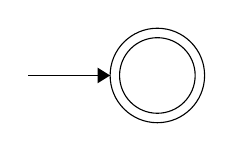
\begin{tikzpicture}[scale=0.2]
        \tikzstyle{every node}+=[inner sep=0pt]
        \draw [black] (26.3,-23.1) circle (3);
        \draw [black] (26.3,-23.1) circle (2.4);
        \draw [black] (18.1,-23.1) -- (23.3,-23.1);
        \fill [black] (23.3,-23.1) -- (22.5,-22.6) -- (22.5,-23.6);
    \end{tikzpicture}

    识别$\epsilon$的FA: \\
    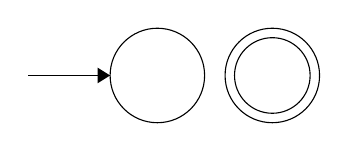
\begin{tikzpicture}[scale=0.2]
        \tikzstyle{every node}+=[inner sep=0pt]
        \draw [black] (26.3,-23.1) circle (3);
        \draw [black] (33.6,-23.1) circle (3);
        \draw [black] (33.6,-23.1) circle (2.4);
        \draw [black] (18.1,-23.1) -- (23.3,-23.1);
        \fill [black] (23.3,-23.1) -- (22.5,-22.6) -- (22.5,-23.6);
    \end{tikzpicture}

    识别$a$的FA: \\
    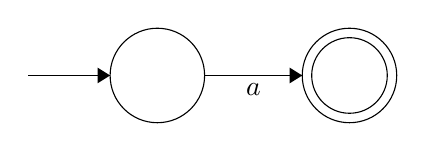
\begin{tikzpicture}[scale=0.2]
        \tikzstyle{every node}+=[inner sep=0pt]
        \draw [black] (26.3,-23.1) circle (3);
        \draw [black] (38.5,-23.1) circle (3);
        \draw [black] (38.5,-23.1) circle (2.4);
        \draw [black] (18.1,-23.1) -- (23.3,-23.1);
        \fill [black] (23.3,-23.1) -- (22.5,-22.6) -- (22.5,-23.6);
        \draw [black] (29.3,-23.1) -- (35.5,-23.1);
        \fill [black] (35.5,-23.1) -- (34.7,-22.6) -- (34.7,-23.6);
        \draw (32.4,-23.6) node [below] {$a$};
        \end{tikzpicture}

    观察得到:上述3个FA具有如下性质:
    \begin{outline}[enumerate]
        \1 有且只有一个终止状态
        \1 没有从终止状态出发的狐
    \end{outline}

    设$M_r, M_S$是$r, s$的具有上述2个性质的FA,则: 

    识别$(r+s)$的FA: \\
    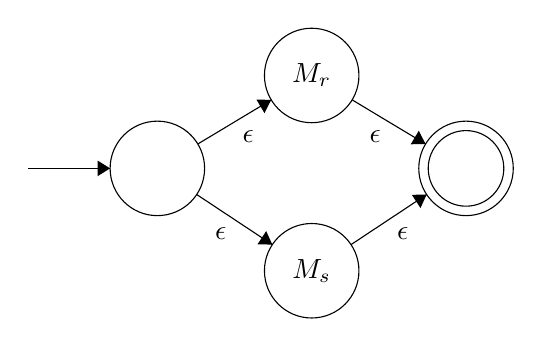
\begin{tikzpicture}[scale=0.2]
        \tikzstyle{every node}+=[inner sep=0pt]
        \draw [black] (26.3,-23.1) circle (3);
        \draw [black] (36.1,-17.2) circle (3);
        \draw (36.1,-17.2) node {$M_r$};
        \draw [black] (36.1,-29.6) circle (3);
        \draw (36.1,-29.6) node {$M_s$};
        \draw [black] (45.9,-23.1) circle (3);
        \draw [black] (45.9,-23.1) circle (2.4);
        \draw [black] (18.1,-23.1) -- (23.3,-23.1);
        \fill [black] (23.3,-23.1) -- (22.5,-22.6) -- (22.5,-23.6);
        \draw [black] (28.87,-21.55) -- (33.53,-18.75);
        \fill [black] (33.53,-18.75) -- (32.59,-18.73) -- (33.1,-19.59);
        \draw (32.07,-20.65) node [below] {$\epsilon$};
        \draw [black] (28.8,-24.76) -- (33.6,-27.94);
        \fill [black] (33.6,-27.94) -- (33.21,-27.08) -- (32.66,-27.92);
        \draw (30.32,-26.85) node [below] {$\epsilon$};
        \draw [black] (38.67,-18.75) -- (43.33,-21.55);
        \fill [black] (43.33,-21.55) -- (42.9,-20.71) -- (42.39,-21.57);
        \draw (40.13,-20.65) node [below] {$\epsilon$};
        \draw [black] (38.6,-27.94) -- (43.4,-24.76);
        \fill [black] (43.4,-24.76) -- (42.46,-24.78) -- (43.01,-25.62);
        \draw (41.88,-26.85) node [below] {$\epsilon$};
    \end{tikzpicture}

    识别$rs$的FA: \\
    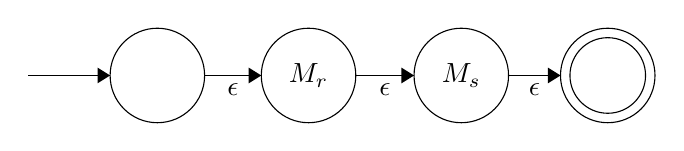
\begin{tikzpicture}[scale=0.2]
    \tikzstyle{every node}+=[inner sep=0pt]
    \draw [black] (26.3,-23.1) circle (3);
    \draw [black] (35.9,-23.1) circle (3);
    \draw (35.9,-23.1) node {$M_r$};
    \draw [black] (45.6,-23.1) circle (3);
    \draw (45.6,-23.1) node {$M_s$};
    \draw [black] (54.9,-23.1) circle (3);
    \draw [black] (54.9,-23.1) circle (2.4);
    \draw [black] (18.1,-23.1) -- (23.3,-23.1);
    \fill [black] (23.3,-23.1) -- (22.5,-22.6) -- (22.5,-23.6);
    \draw [black] (29.3,-23.1) -- (32.9,-23.1);
    \fill [black] (32.9,-23.1) -- (32.1,-22.6) -- (32.1,-23.6);
    \draw (31.1,-23.6) node [below] {$\epsilon$};
    \draw [black] (38.9,-23.1) -- (42.6,-23.1);
    \fill [black] (42.6,-23.1) -- (41.8,-22.6) -- (41.8,-23.6);
    \draw (40.75,-23.6) node [below] {$\epsilon$};
    \draw [black] (48.6,-23.1) -- (51.9,-23.1);
    \fill [black] (51.9,-23.1) -- (51.1,-22.6) -- (51.1,-23.6);
    \draw (50.25,-23.6) node [below] {$\epsilon$};
    \end{tikzpicture}

    识别$r^*$的FA: \\
    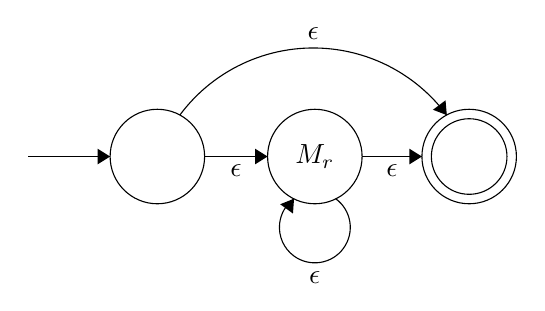
\begin{tikzpicture}[scale=0.2]
        \tikzstyle{every node}+=[inner sep=0pt]
        \draw [black] (26.3,-23.1) circle (3);
        \draw [black] (36.3,-23.1) circle (3);
        \draw (36.3,-23.1) node {$M_r$};
        \draw [black] (46.1,-23.1) circle (3);
        \draw [black] (46.1,-23.1) circle (2.4);
        \draw [black] (18.1,-23.1) -- (23.3,-23.1);
        \fill [black] (23.3,-23.1) -- (22.5,-22.6) -- (22.5,-23.6);
        \draw [black] (29.3,-23.1) -- (33.3,-23.1);
        \fill [black] (33.3,-23.1) -- (32.5,-22.6) -- (32.5,-23.6);
        \draw (31.3,-23.6) node [below] {$\epsilon$};
        \draw [black] (39.3,-23.1) -- (43.1,-23.1);
        \fill [black] (43.1,-23.1) -- (42.3,-22.6) -- (42.3,-23.6);
        \draw (41.2,-23.6) node [below] {$\epsilon$};
        \draw [black] (27.724,-20.471) arc (143.41431:36.58569:10.556);
        \fill [black] (44.68,-20.47) -- (44.6,-19.53) -- (43.8,-20.13);
        \draw (36.2,-15.71) node [above] {$\epsilon$};
        \draw [black] (37.623,-25.78) arc (54:-234:2.25);
        \draw (36.3,-30.35) node [below] {$\epsilon$};
        \fill [black] (34.98,-25.78) -- (34.1,-26.13) -- (34.91,-26.72);
    \end{tikzpicture}
\end{proof}

\begin{theorem}
    对于$\forall$ RE $r, \exists$ FA $M$,使得$L(M) = L(r)$
\end{theorem}

\section{正则语言的性质}
\subsection{正则语言的泵引理}
\begin{example}
    如何证明$L = \set{0^n1^n |n \ge 1}$ 不是RL?

    假设$L$是RL。DFA $M = (Q, \Sigma, \delta, q_0, F)$ 使得$L(M) = L$。

    记$|Q| = N,\; N \ge 1$,取$0^n1^n \in L, n \ge N$。

    设$q_i$为$M$读取$0^n1^n$的前$i$位时的状态。注意到$n \ge N$,所以在
    $q_0, q_1, \dots, q_n$中至少有两个重复状态。不妨设$q_i = q_j$是最早重复
    的状态。则$0 \le i,j \le N$。

    所以:
    \begin{outline}
        \1 $\delta(q_0, 0^i) = q_i$
        \1 $\delta(q_i, 0^{j-i}) = q_j$
        \1 $\delta(q_j, 0^{n-j}1^n) = q_2n \in F$
    \end{outline}

    所以:$\delta(q_i, {(0^{j-i})}^k) = q_i = q_j$。
    也就是说,对于$\forall k \ge 0$,$\delta(q_0, 0^i{(0^{j-i})}^k0^{n-j}1^n) \in F$
\end{example}

\begin{lemma}
    正则语言的的泵引理。对于$\forall\; RL\; L$,存在一个仅依赖与$L$的正整数$N$,对于$\forall z
    \in L, |z| \ge N$,则存在$u, v, w$满足以下条件:
    \begin{outline}
        \1 $uvw = z$
        \1 $|uv| \le N$
        \1 $|v| \ge 1$
        \1 对于$\forall k \ge 0$,$uv^kw \in L$
    \end{outline}
\end{lemma}

\begin{lemma}
    拓展的泵引理。对于$\forall\; RL\; L$,存在一个仅依赖与$L$的正整数$N$,对于$\forall z = z_1z_2z_3
    \in L, |z_2| \ge N$,则存在$u, v, w$满足以下条件:
    \begin{outline}
        \1 $uvw = z_2$
        \1 $|uv| \le N$
        \1 $|v| \ge 1$
        \1 对于$\forall k \ge 0$,$uv^kw \in L$
    \end{outline}
\end{lemma}

\begin{example}
    证明$L=\set{0^p|p\text{是质数}}$不是RL。

    设$L$是RL。$N$是泵引理所说正整数。设$x$为大于$N$的最小质数。

    取$z = 0^x$。取$v = 0^l,\; l \ge 1$。$uv^kw = 0^{x+(k-1)l}$。

    当$k = x+1$时,有$x+(x+1-1)l = (l+1)x$是合数,所以$uv^kw \notin L$,与泵引理矛盾。

    所以L不是RL。
\end{example}

\begin{example}
    设$L = \set{0^{2n} | n \ge 1}$,证明L不是RL。

    假设N是仅依赖于L的正整数。取$z = 0^{2N}$,取$u = 0^l$, $v = 0$, $w = 0^{2N - l - 1}$。

    $uv^kw = 0^{2N + (k-1)}$ 当$k = 0$时,$uv^kw = 0^{2N - 1} \ne L$。

    与泵引理矛盾,所以L不是RL。

    \hl{证明错误!不能取$v = 0$,要让$\forall v $矛盾!}
\end{example}
\subsection{RL的封闭性}
\begin{theorem}
    RL对于并、乘、闭包封闭。

    证明: 根据正则表达式的定义,定理显然成立。\qed
\end{theorem}
\begin{theorem}
    RL对补运算封闭。

    证明:把对应的DFA的F取反,可构造新的DFA,可构造新的RL。\qed
\end{theorem}
\begin{theorem}
    RL对交运算封闭。

    证明:$L1 \cup L2 = \overline{\overline{L1} \cap \overline{L2}}$\qed
\end{theorem}

\subsection{Myhill定理}
\begin{definition}
    $\begin{aligned}[t]
        x R_M y & \iff \delta(q_0, x) = \delta(q_0, y) \\
            & \iff \exists q \in Q, x, y \in set(q)
    \end{aligned}$
\end{definition}
\begin{definition}
    $\begin{aligned}[t]
        x R_L y & \iff \forall z \in \Sigma^*, xz \in L \iff yz \in L
    \end{aligned}$
\end{definition}
\begin{definition}
    R是右不变的是指如果$xRy$则有$\forall z \in \Sigma^*, xzRyz$
\end{definition}
\begin{theorem}
    对于DFA M,如果$x R_M y$,则$x R_{L(M)} y$。
    
    证明:由$x R_M y$知$\delta(q_0, x) = \delta(q_0, y)$。不妨设其为
    $q_1$。

    对于$\forall z \in \Sigma^*$,$\delta(q_0, xz) =  \delta(\delta(q_0, x), z) = \delta(q_1, z) 
    = \delta(q_0, yz)$。不妨设其为$q_2$。

    如果$xz \in L$,则有$q_2 \in F$,所以$yz \in L$。反之亦然。

    所以 $xz \in L \iff yz \in L$。
    所以 $x R_M y \iff x R_{L(M)} y$
    \qed
\end{theorem}

\begin{theorem}
    Myhill定理。以下3个命题等价:
    \begin{outline}[enumerate]
        \1 L 是 RL
        \1 L 是 $\Sigma^*$上的某个具有有穷指数的右不变等价关系的某些等价类的并。
        \1 $R_L$ 具有有穷指数。
    \end{outline}

    \begin{proof}
        $1 \Rightarrow 2$。

        设L是RL,DFA M使得$L(M) = L$。

        $R_M$是$\Sigma^*$上的右不变等价关系,且$|\Sigma^* / R_M| \le |Q|$。

        $\displaystyle L = \bigcup_{q \in F}set(q)$
    \end{proof}

    \begin{proof}
        $2 \Rightarrow 3$。

        设$L$是$\Sigma^*$上的具有有穷指数的右不变等价关系$R$的某些等价类的并。

        下面证明如果$x R y$,那么$x R_L y$。

        设$x, y \in \Sigma^*, xRy$。由$R$的右不变性,对于$\forall z \in \Sigma^*$,$xzRyz$。

        再注意到$L$是$R$的某些等价类的并,且$xz,yz$在同一个等价类中,所以$xz \in L \iff yz \in L$。
        
        所以$x R_L y$。
    \end{proof}

    \begin{proof}
        $3 \Rightarrow 1$。
        
        设$R_L$具有有穷指数。取$M' = (\Sigma^*/R_L, \Sigma, \delta', [\epsilon], \set{[x] | x \in L})$

        $\delta'([a], x) = [ax]$。显然,$L(M') = L$。
    \end{proof}
\end{theorem}

\hl{意义:L是RL的充要条件}

\begin{theorem}
    在同构意义下,$M'$是状态最少的唯一识别L的DFA。
\end{theorem}

\subsection{DFA的最小化}
用极小化算法得到的DFA去掉不可达状态后得到的DFA为状态最少的DFA。

\begin{outline}
    \1 寻找可以(应该)合并的类/状态
    \1 算法实现: \\
        找出所有不可合并的类
\end{outline}
\subsubsection{证明L 是/不是 RL}
\begin{outline}[enumerate]
    \1 证明L是RL。

        证明$R_L$的指数有穷。
    \1 证明L不是RL:
        
        证明$R_L$的指数无穷。
\end{outline}
\begin{example}
    证明 $\set{0^n1^m|n,m \ge 1}$ 是RL。

    $R_L$的指数应该有穷。首先分析L的特征:
    \begin{outline}[enumerate]
        \1 0和1的个数非0。
        \1 0不能出现在1后面。
    \end{outline}

    故,分成如下几类:

    \begin{outline}[enumerate]
        \1 0在1后面($\set{x | x\text{中有子串}10}$)
        \1 $\set{0^n1^m | n,m \ge 1}$
        \1 $\set{\epsilon}$
        \1 $1^n$
        \1 $0^n$
    \end{outline}

    观察发现,1和5可以合并,因此得到:

    $\Sigma^* / R_L = \set*{[\epsilon], [0], [01], [10]}$。$R_L$的
    指数为4,所以L是RL。
\end{example}
\begin{example}
    证明 $\set{0^n1^n | n \ge 0}$ 不是RL。

    易得,对于$\forall i \ne j \in N$,$0^i \cancel{R_L} 0^j$
    因此$R_L$的指数无穷。
\end{example}
\section{CFL 上下文无关语言}
\subsection{CFG}
\begin{definition}
    CFG $G=(V, T, P, S)$的语法树为满足如下条件的树:

    \begin{outline}[enumerate]
        \1 每个节点的标记$x \in V \cup T \cup \set{\epsilon}$
        \1 如果节点V的标记为$A$,V从左到右的子节点$V_1,V_2,\dots,V_k$
        的标记依次为$y_1,y_2,\dots,y_k$,则$A \to y_1y_2\dots y_k \in P$
        \1 根节点标记为S
        \1 中间节点的标记为变量$x \in V$
        \1 从左到右的叶子节点$v_1,\dots,v_n$的标记$x_1,\dots,x_n$
        组成的串$x_1x_2\dots x_n$为该树的结果。
        \1 如果v的标记为$\epsilon$,则它没有兄弟。
        % \1 如果节点V的标记为终结符号,则它是叶子节点。
    \end{outline}
\end{definition}
\begin{example}
    $X \to (S) | S | \epsilon$,请画出句型$((S))$的语法树。
\end{example}
\begin{definition}
    满足语法树定义中除第三条外条件的树,称作A-子树。
\end{definition}
\begin{theorem}
    有一颗结果为$\alpha$的语法树$\iff S \overset{*} \Rightarrow \alpha $
\end{theorem}
\begin{definition}
    每一步派生均实施在当前句型最右变量上的派生叫最右派生。

    每一步派生均实施在当前句型最左变量上的派生叫最左派生。
\end{definition}
\begin{theorem}
    最左派生与最右派生的语法树是一一对应的。
\end{theorem}
\begin{definition}
    如果CFG G有句子有棵颗不同的语法书,则G是二义性的。
\end{definition}
\begin{definition}
    如果CFL L没有非二义性文法,则称之为固有二义性的。
\end{definition}
\subsection{去无用符号}

\subsubsection{去除无用符号}
\begin{definition}
    X是有用符号,即$\exists X \in L(G)$,$S \overset{*} \Rightarrow
    \alpha X \beta \overset{*} \Rightarrow x$。

    X是有用的,必须同时满足如下两条:
    \begin{outline}[enumerate]
        \1 $S \overset{*} \Rightarrow \alpha X \beta$
            
            如何判断?

            \2 $V' = \set{S} \cup \set{A | S \to \alpha A \beta \in P}$

                $T' = \set{a | S \to \alpha a \beta \in P}$
            \2 重复 \\
            $V' = V' \cup \set{B | A \to \alpha B \beta \in P \& A in V'}$ \\
            $T' = T' \cup \set{a | A \to \alpha a \beta \in P \& A in V'}$
        \1 $X \overset{*} \Rightarrow w, w \in T^*$
        
            $G = (V, T, P, S)$,对于:

            $\forall a \in T$,$a$满足2。
        
            $\forall A \in V$,如何判断$A$是否满足2?
            % \begin{outline}[enumerate]
                \2 $V' = \set{A | A \to w \in P}$
                \2 重复 $V' = \set{A | A \to \alpha, \alpha \in (V' \cup T)^*} \cup V'$
        % \end{outline}
    \end{outline}
\end{definition}
\begin{theorem}
    对于$\forall$ CFG G,$\exists$ CFG $G'$,
    \begin{outline}[enumerate]
        \1 $L(G') = L(G)$
        \1 $G'$中无无用符号。
    \end{outline}
\end{theorem}


\subsubsection{去除$\epsilon-$产生式}
\begin{definition}
    如果$A \overset{*} \Rightarrow \epsilon$,则称A为可空变量。
\end{definition}
\begin{theorem}
    对于$\forall$ CFG $G, G'$:
    \begin{outline}[enumerate]
        \1 $G'$中无空产生式
        \1 $L(G') = L(G) - \set{\epsilon}$
    \end{outline}
    对于$A \to x_1x_2\dots x_n$,替换为$A \to y_1y_2\dots y_n$,其中
    当$x_i$不是可空变量时,$y_i = x_i$,否则$y_i = x_i$或$\epsilon$。

    注意$y_1y_2\dots y_n$不能都为$\epsilon$。
\end{theorem}

\subsubsection{去单一产生式}
\begin{definition}
    形如$A \to B$的产生式是单一产生式。
\end{definition}
\begin{definition}
    对$\forall$ CFG G,$\exists$ CFG $G', L(G') = L(G)$,$G'$中无单一产生式。

    推论:对于$\forall$ CFG $G$, 存在$CFG$ G' 使得$L(G') = L(G)$,且$G'$没有无用符,$\epsilon -$产生式和单一产生式。
\end{definition}

\subsection{CNF 乔姆斯基范式}
\begin{definition}
    如果G的产生式均具有以下形式:
    
    $$
    \begin{cases}
        A \to BC \\
        A \to a
    \end{cases}
    $$

    则称之为CNF。
\end{definition}
\subsection{GNF 格雷巴赫范式}
\begin{definition}
    如果G的产生式均具有以下形式:
    
    $$
        A \to a\alpha, \alpha \in V^*
    $$

    则称之为GNF。
\end{definition}

\begin{example}
    $A \to Aa | b = \begin{cases}
        A \to b | bB \\
        B \to a | aB
    \end{cases}$
\end{example}

\begin{example}
    $A \to Aa | Ab | c | d = \begin{cases}
        A \to c | d | cB | dB \\
        B \to a | b | aB | bB
    \end{cases}$
\end{example}
\begin{example}
    $
        A \to  A\alpha_1 | A\alpha_2 | A\alpha_3 | \beta_1 | \beta_2 
        = \begin{cases}
            A \to \beta_1 | \beta_2 | \beta_1B | \beta_2B \\
            B \to \alpha_1 | \alpha_2  | \alpha_3 | \alpha_1B | \alpha_2B | \alpha_3B
        \end{cases}
    $
\end{example}

\begin{example}
    $
        \begin{cases}
            S \to ABS | BAA \\
            A \to BB | BAA \\
            B \to aB | b
        \end{cases} = \begin{cases}
            S \to aBBBS | bBBS | aBAABS | bAABS 
                    aBAA | bAA\\
            A \to aBB | bB | aBAA | bAA \\
            B \to aB | b
        \end{cases}
    $
\end{example}

步骤:
\begin{outline}[enumerate]
    \1 给变量排序
    \1 从$A_1$到$A_n$逐一使产生式满足如下要求:

    $A_i \to A_h \alpha, j \ge i$
    \1 从$A_{n-1}$开始通过回代,逐一使$A_{n-1},A_{n-2}\dots$的产生式满足要求
    \1 通过代入,使第二步中引入的新变量的产生式满足要求。

    关键: \hl{去左递归}

    如:

    $$
    \begin{cases}
        A \to A\alpha_1 | A\alpha_2 | \dots | A\alpha_n \\
        A \to \beta_1 | \beta_2 | \dots | \beta_m
    \end{cases}
    $$
    为所有A产生式,且$\beta_1, \beta_2, \dots, \beta_m$的首字母不是A,可以用如下的产生式组替代:
    $$
    \begin{cases}
        A \to \beta_1 | \beta_2 | \dots | \beta_m | \beta_1 A' | \beta_2 A' | \dots | \beta_, A' \\
        A' \to \alpha_1 A' | \alpha_2 A' | \dots | \alpha_n A' | \alpha_1 | \alpha_2 | \dots | \alpha_n
    \end{cases}
    $$
\end{outline}
\begin{theorem}
    对于$\forall$化简了的CFG,$\exists$ GNF 与之等价。
\end{theorem}

\section{PDA 下推自动机}
\subsection{PDA的定义}
\begin{definition}
    PDA $M = (Q, \Sigma, \Gamma, \delta, q_0, z_0, F)$
    其中:
    \begin{description}
        \item[$Q$]:状态的有穷集合
        \item[$\Sigma$]: 输入字母表
        \item[$\Gamma$]: 栈符号的非空有穷集
        \item[$\delta$]: 状态转义函数\\
            $Q\times (\Sigma \cup \set{\epsilon}) \times \Gamma \to 2^{Q \times \Gamma^*} $。 
            
            $\forall (q,a,A) \in Q\times (\Sigma \cup \set{\epsilon}) \times \Gamma$,
            $\delta(q,a,A) = \set{(p_1,\gamma_1),\dots,(p_k,r_k)}$表示$M$在状态$q$,栈顶为$A
            $时读到$a$,将栈顶符号$A$弹出,将$\gamma_i$依次压入栈,并将状态改为$p_i$。

            $\forall (q,A) \in Q\times \Gamma$,
            $\delta(q,\epsilon,A) = \set{(p_1,\gamma_1),\dots,(p_k,r_k)}$表示$M$在状态$q$,栈顶为$A
            $时做空移动,将栈顶符号$A$弹出,将$\gamma_i$依次压入栈,并将状态改为$p_i$。
        \item[$q_0$]:开始状态
        \item[$z_0 \in \Gamma$]:栈底符号
        \item[$F$]: 终止状态 
    \end{description}
\end{definition}

\begin{definition}
    PDA M的ID $(q, x, \alpha) = Q \times \Sigma^* \times \Gamma^*$

    其中 $q$ 是M的当前状态, $x$是M的输入带上剩余串,$\alpha$是M的栈中当前的内容。

    设M当前的ID是$(q, ax, A\alpha)$,如果$(p, \gamma) \in \delta(q, a, A)$,则M的ID变为$(p, x, \gamma \alpha)$,记作$(q, ax, A\alpha) \vdash_M (p, x, \gamma\alpha)$。

    如果$(p, \gamma) \in \delta(q, \epsilon, A)$,则M的ID变为$(p, ax, \gamma \alpha)$,记作$(q, ax, A\alpha) \vdash_M (p, ax, \gamma\alpha)$。
    
    $\vdash_M$ 是 $Q \times \Sigma^* \times \Gamma^*$上的二元关系。
\end{definition}

\begin{definition}
    $M = (Q, \Sigma, \Gamma, \delta, q_0, z_0, F)$

    用终态识别的语言$L(M) = {x | (q_0, x, z_0) \vdash^* (q, \epsilon, \alpha) \text{ and } q \in F}$。

    用空栈识别的语言$N(M) = {x | (q_0, x, z_0) \vdash^* (q, \epsilon, \epsilon) \text{ and } q \in F}$。
\end{definition}

\end{document}
